% All the result and analysis
\chapter{Results and Analysis}

\section{Initial configuration with two prey species}

% Put the table here
\begin{table}
\centering
\caption{Agent configuration of 2 prey species}
\label{tab:config-table-2-prey}
\begin{tabular}{|l|l|c|c|l|c|}
  \hline
   														&\multicolumn{3}{|c|}{Prey configuration} 																	
   														& \multicolumn{2}{|c|}{Predator configuration} \\ \hline
  \multirow{2}{*}{Population} & Rule110 (Palatable) & 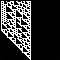
\includegraphics[scale=0.50]{images/CARule110} & 108 
  														& \multicolumn{2}{|c|}{\multirow{2}{*}{10}} \\ \cline{2-4}
  					 									& Rule30 (Unpalatable)& 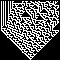
\includegraphics[scale=0.50]{images/CARule30}  & 108 
  					 									& \multicolumn{2}{|c|}{}\\ \hline
  \multirow{2}{*}{Reproduction} & Age Limit & \multicolumn{2}{|c|}{100}  & \multicolumn{2}{|c|}{500} \\ \cline{2-6}
  						 									& Interval  & \multicolumn{2}{|c|}{1000} & \multicolumn{2}{|c|}{1000} \\ \hline
  \multirow{2}{*}{Mutation Rate} & Pattern   & \multicolumn{2}{|c|}{0.05} & \multicolumn{2}{|c|}{\multirow{2}{*}{0.03}} \\ \cline{2-4}
  						 									 & Genome    & \multicolumn{2}{|c|}{0.5}  & \multicolumn{2}{|c|}{} \\ \hline
  Demise Age	 									 & \multicolumn{3}{|c|}{2000}							& \multicolumn{2}{|c|}{2500} \\ \hline
  Minimum Attack Age						 & \multicolumn{3}{|c|}{} 						    & \multicolumn{2}{|c|}{500} \\ \hline
  \multirow{2}{*}{Memory Configuration} & \multicolumn{3}{|c|}{} 					& Minimum & 2 \\ \cline{5-6}
   																			& \multicolumn{3}{|c|}{} 					& Maximum & 10 \\ \hline  
\end{tabular}
\end{table}

\paragraph{}
The set of parameters in Table \ref{tab:config-table-2-prey} were carefully selected to be the initial condition for this run of the simulation. This test has been done with two sets of prey species with very different CA pattern and with opposite palatability and equal population. To control reproduction of the prey species their age limit has been set to 100 iterations into the time the species were alive. And the reproduction interval was set to 1000 iterations.

\paragraph{}
Pattern mutation rate has been set to a minimal level of 0.05 as by increasing this variable it is possible to increase the size of the number of mimicry rings present in the simulation. The Genome mutation rate controls the rate at which genome of the child prey species will deviate from their parents. As mentioned earlier the genome mutation rate has been separated from the pattern mutation rate to bring more control to the number of mimicry rings generated.

\paragraph{}
Prey demise age has been kept to 2000 iterations while predator demise age is set to 2500. But later in the following results predator demise age has been increased to 5000 iterations. Predators in this simulation generates selection pressure for the evolution of mimicry. So the longer a predator is present in the simulation it will be making intelligent decisions in term of selecting which prey species to consume and which one to avoid. But with the current rate of demise for predator we were able to create successful mimetic population of prey species as we will see in the analysis in the following results.

\paragraph{}
Initial population of predator species has been set to 10 which is in accordance with the prey population in the simulation. The reason for such low number of predator is, unlike prey species which are consumed by predators, there is no cause for the predator species to die accept their natural cause of death, that is to reach their demise age. So predator population can explode very easily. That is why their population is controlled in a restrictive manner with the help of high reproduction age limit and reproduction age interval.

\paragraph{}
The memory configuration size for predators are a very interesting parameter. The minimum memory size is directly associated with the number of prey species with which we initiate the simulation. Otherwise evolution of mimicry is not observed. As mentioned earlier the minimum memory size is the number of prey species predator would consume before starting to make decisive consumption of prey species. After the initial birth of a predator and when the minimum attack age is crossed, it starts consuming prey species present in its vicinity without making any judgement. At this point its memory size is zero. As long as the minimum memory size is not reached predators will blindly consume prey species and insert their CA pattern and associated palatability into its Hopfield memory bank. No later than the minimum memory size has been reached, predators will start making intelligent decision about consuming its prey species. When catching a prey if its memory tells that it is palatable, it will consume that prey. Otherwise if memory recognizes it to be unpalatable predator will certainly let it go.

\paragraph{}
Now as we know the behaviour of Hopfield memory, a recognition result will always be achieved depending on the similarity of the patterns stored in memory. So when minimum memory size has been reached the predator will always make a decision based on the similarity of the prey pattern previously captured and the patterns stored in memory.

% Put the image
\begin{figure}
	\centering
	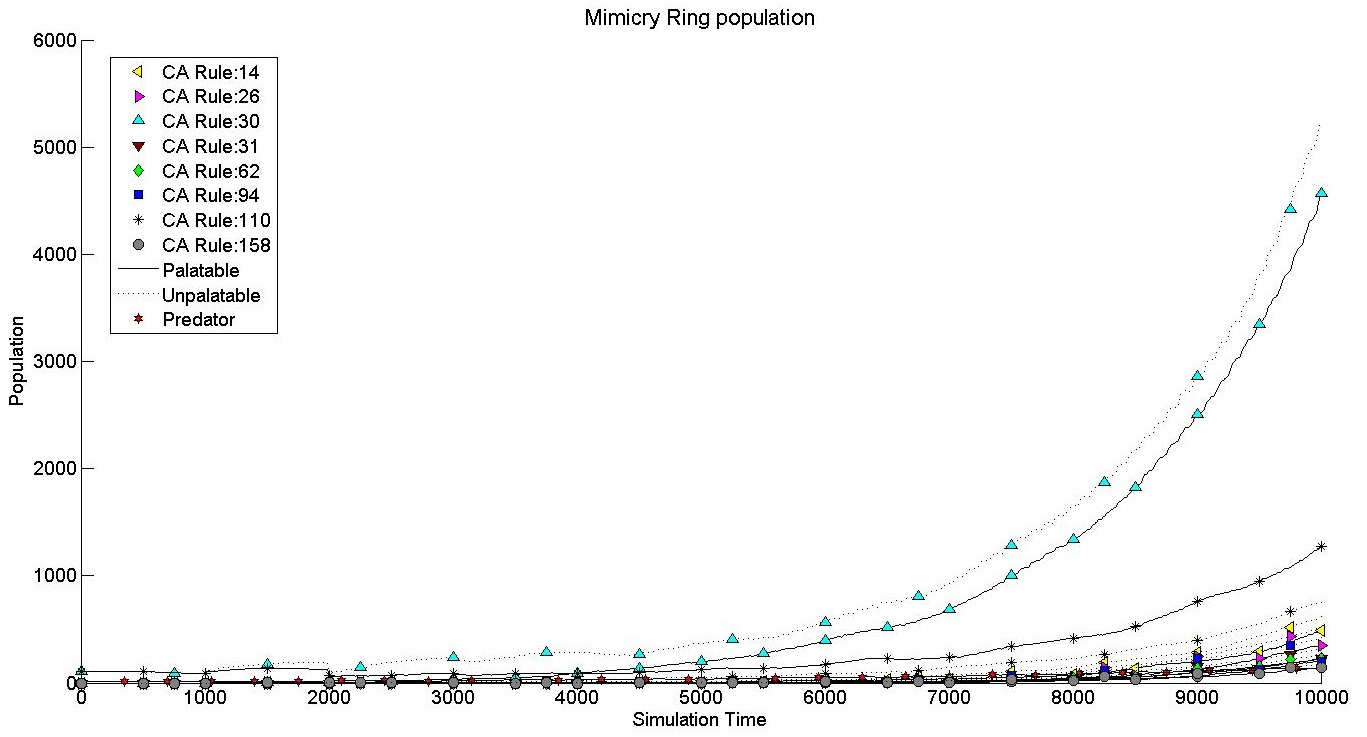
\includegraphics[scale=0.40]{images/simTime10k-2Prey}
	\caption{Population distribution of mimicry rings, initialized with 2 prey species.}
	\label{fig:plot-2-prey}
\end{figure}

\paragraph{}
The plot in Figure \ref{fig:plot-2-prey} is simulation time verses prey population after running it for above 10000 iterations. With the initial configuration in the above table we can observe that multiple rings of prey population has been created. Two prey species are in a ring if their CA pattern have a hamming distance within 10 bits. Population of palatable species has been represented with line curve while population of unpalatable species has been presented with dotted curve. Different signs of squares, triangles and diamonds have been used to distinguish between species of prey population. The simulation was initiated with two prey species having CA rule of 30 and 110 and being palatable and unpalatable consecutively.

\paragraph{}
By closely observing the graph we could see the population of two species have started dropping at around time 500 when the initial predator population reaches this maturity for consuming prey species. At around time 1000 the prey population starts reproducing as the population increases. At around the same time different other species of prey population gets to be born with mutated CA patterns. Over time the population of CA Rule 110 dominates the population as most predators recognizes it as unpalatable. And similarly a population of CA Rule 110 or within the same ring of palatable species starts rising, while at one point overlaps the population of CA Rule 30 (Time: 5000 approx.) which was initially considered as a set of palatable species.

\paragraph{}
We can observe from the above results that the evolution of mimicry has taken effect. A population of mimics were successfully able to exceed the population of other prey species the reason being avoidance by predators of prey pattern similar to unpalatable ones. We can conclude that Batesian mimicry has taken effect in the simulation.

\paragraph{}
The above configuration in Table \ref{tab:config-table-2-prey} is also the most appropriate condition for Mullerian Mimicry. We can observe that a single pattern of unpalatable species dominate the entire population. These effects can be observed in this configuration where we can see the continuous increment of prey and predator population and eventually behaviors of Mullerian mimicry, where all prey species converge to a single ring of CA pattern.

%Put the number of rings picture:
\begin{figure}
	\centering
	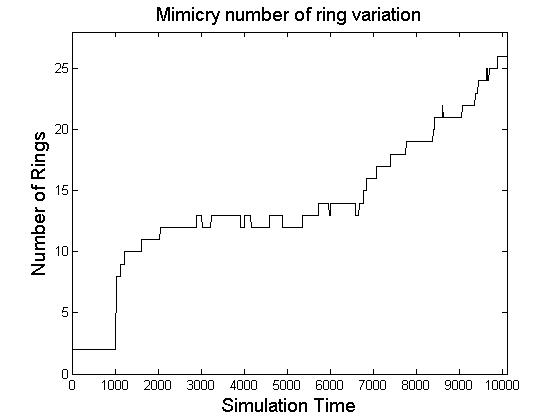
\includegraphics[scale=0.40]{images/ringSize10k-2Prey}
	\caption{Number of mimicry rings, initialized with 2 prey species.}
	\label{fig:ringSize10k-2Prey}
\end{figure}

\paragraph{}
As it can be observed from Figure \ref{fig:ringSize10k-2Prey} the number of rings in this simulation makes a slow increase from 2 at the initial configuration to 33 rings at the end of 10000 iterations. We can observe that a small change in CA genetic representation can have a very large effect in terms of the phenotype of the pattern with which the prey is represented. For example if we observe the following set of patterns genotype with very different phenotype:

%CARule table
\begin{table}
\centering
\caption{Difference in prey pattern genotype and phenotype}
\label{tab:diff-in-pattern}
\begin{tabular}{|l|c|c|c|}
  \hline
  CA Rule & \(60 \equiv 00111100\) & \(61 \equiv 00111101\) & \(62 \equiv 00111110 \) \\ \hline
  Pattern & 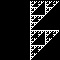
\includegraphics[scale=0.50]{images/CARule60} & 
\includegraphics[scale=0.50]{images/CARule61} & 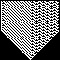
\includegraphics[scale=0.50]{images/CARule62}\\
  \hline
\end{tabular}
\end{table}

\paragraph{}
All the patterns in Table \ref{tab:diff-in-pattern} have a genetic bit difference of 1. So by a single mutation there can be three different set of phenotype for a child organism from its parent. This is largely the reason for the increased number of Rings created in the simulation. Only the 8 most populous rings have presented in the graph above with population verses simulation time.

%Screenshot of the simulation
\begin{figure}
	\centering
	\label{fig:screenshot-simTime7600-2-prey}
	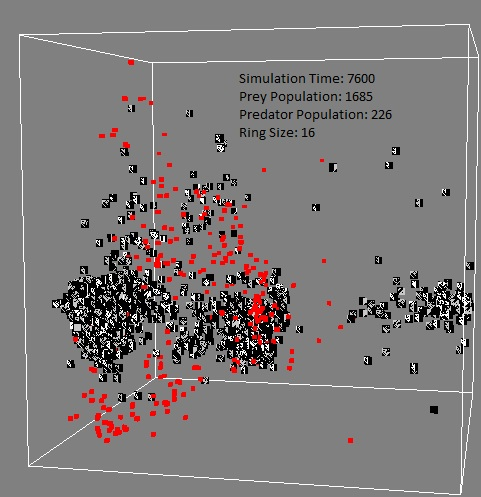
\includegraphics[scale=0.65]{images/simTime7600}
	\caption{Graphical representation of the model, simulation time: 7600.}
\end{figure}

\paragraph{}
The screen shot in Figure \ref{fig:screenshot-simTime7600-2-prey} is for one instance of time of the simulation. The red agents are predators while the black agents with different textured patterns are the prey species. According to their behavior most of the prey species are flocking together in a group while also being chased by the predators, whose sole purpose is to consume prey species. 

\section{Initial configuration with four prey species}

\paragraph{}
\paragraph{}
\paragraph{}
\paragraph{}
\paragraph{}
\paragraph{}
\paragraph{}
